\documentclass[a4paper]{article}
\usepackage[warn]{mathtext}
\usepackage[utf8]{inputenc}
\usepackage[T2A]{fontenc}
\usepackage[english,russian]{babel}
\usepackage{indentfirst}
\usepackage{misccorr}
\usepackage{subcaption}
\captionsetup{compatibility=false}
\usepackage{geometry}
\geometry{verbose,a4paper,tmargin=2cm,bmargin=2cm,lmargin=1.5cm,rmargin=1.5cm}
\usepackage{graphicx}
\usepackage{wrapfig}
\usepackage{amsmath}
\usepackage{fancyhdr}
\usepackage{floatflt}
\usepackage{float}
\usepackage{amssymb}
\usepackage{color}
\usepackage{lscape}
\usepackage{hvfloat}
\usepackage{amsfonts}
\usepackage{euscript}
\usepackage{newunicodechar}
\usepackage{booktabs}

\begin{document}
\newcommand{\apple}{\char"F8FF}

\begin{titlepage}
  \vspace*{4cm}
\centering
  {\scshape\LARGE Московский физико-технический институт\par}
\vspace{1cm}
{\scshape\Large Лабораторная работа по общей физике № 1.3\par}
\vspace{1cm}
  {\huge\bfseries  Эффект Рамзауэра - изучение рассеяния медленных электронов на атомах.\par}
\vspace{2cm}
\vfill
\begin{flushright}
{\large Выполнила студентка Б01-907}\par
\vspace{0.3cm}
{\LARGE Юлия Прохорова}
\end{flushright}

\vfill
Долгопрудный, 2021
% Bottom of the page
\end{titlepage}

\pagestyle{fancy} 
\fancyhead[L]{№ 1.3}
\fancyhead[R]{Юля Прохорова, Б01-907}
\fancyhead[C]{}
\fancyfoot[C]{ \noindent\rule{\textwidth}{0.4pt} \thepage }

\tableofcontents

\newpage

\section{Цель работы} Исследовать энергетическую зависимость вероятности рассеяния электронов атомами инертного газа,
 определить энергию электронов, при которой наблюдается <<просветление>> инертного газа и оценить размер его внешней электронной оболочки.

\section{Оборудование} Тиратрон ТГ3-01, источник питания, электронный осциллограф, вольтметр, амперметр.

\section{Теория}
Качественно эффект Рамзауэра наблюдался на примере аргона: при уменьшении энергии электрона поперечное сечение упругогорассеяния ($\sigma = \frac{N}{nv}$) растет - чем меньше скорость электрона, тем медленне он проскакивает мимо атома, тем больше времени атом и электрон взаимодействуют, а, значит, и вероятность взаимодействия растет. Однако в эксперименте с аргоном при энергиях менее $16эВ$ сечение начинает уменьшаться, а при $1эВ$ практически нулевое. При дальнейшем уменьшении энергии сечение рассеяния опять возрастает.
\\
Объяснение эффекта потребовало учета волновой природы электронов.  Поучок электронов, вылетая из накаленного атода, проходит ускоряющую разность потенциалов между катодом и электродом и преобретает $E=\frac{mv^2}{2}=eV$. При прохождении через газ часть электронов рассеивается на атомах, уходит в сторону и собирается электродом, остальные же попадают на анод и создают анодный ток $I$, который пропорционален числу вошедших электронов.

\begin{figure}[H]
  \begin{center}
  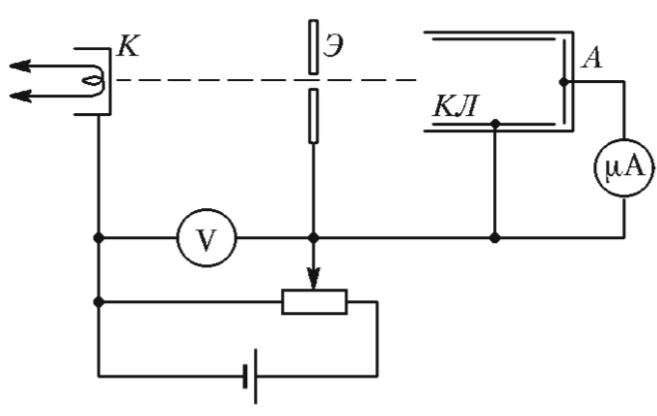
\includegraphics[scale = 0.5]{схема.png}
  \caption{Схема установки для измерения сечения рассеяния электронов в газах}
  \end{center}
\end{figure}

При столкновении с атомом скорость электрона меняется, а, значит, меняется и длина его волны де Бройля. Следовательно для электронной волны газ - преломяющая среда с $n = \frac{\lambda}{\lambda'}= \sqrt{1 - \frac{U}{E}}$, $U$ - потенциальнаяэнергия налетающего электрона, $\lambda = \frac{h}{mv}$.

Рассеяние электрона на атоме можно приближённого рассматривать как рассеяние частицы энергии $E$ на потенциальной яме шириной $\ell$ и глубины $U_0$. Уравнение Шрёдингера имеет вид
\[\Psi'' + k^2 \Psi = 0,\]
где вне ямы 
\[k^2 = k_1^2 = \dfrac{2mE}{\hbar^2},\]
а внутри 
\[k^2 = k_2^2 = \dfrac{2m(E+U_0)}{\hbar^2}.\]
Коэффициент прохождения в таком случае равен
\[D = \dfrac{16 k_1^2 k_2^2}{16k_1^2 k_2^2 + 4(k_1^2 - k_2^2)^2\sin^2(k_2\ell)}.\]
Заметим, что коэффициент прохождения имеет ряд максимумов и минимумов. Он максимальнем при
\begin{equation}\label{0}
\sqrt{\dfrac{2m(E+U_0)}{\hbar^2}}\ell = n\pi,~n=1,2,3,\dots
\end{equation}

Это условие легко получить, рассмотрев интерференцию прошедшей и дважды отразившейся от оболочки волн де Бройля. 
\[\lambda = \dfrac{h}{\sqrt{2mE}},~\lambda_1 = \dfrac{h}{\sqrt{2m(E+U_0)}}.\]
Соответственно условия на первые интерфереционные максимум и минимум 
\begin{equation}\label{1}
2\ell = \dfrac{h}{\sqrt{2m(E_1 + U_0)}},~2\ell = \dfrac{3}{2}\dfrac{h}{\sqrt{2m(E_2 + U_0)}}.
\end{equation}
Исключая из этих соотношений глубину ямы, получим
\begin{equation}\label{2}
\ell = \dfrac{h\sqrt{5}}{\sqrt{32m(E_2 - E_1)}}.
\end{equation}
Глубина ямы при этом равна
\begin{equation}\label{4}
U_0 = \dfrac{4}{5}E_2 - \dfrac{9}{5}E_1.
\end{equation}

\section{Экспериментаьная установка}
\begin{figure}[h]
    \subfloat{{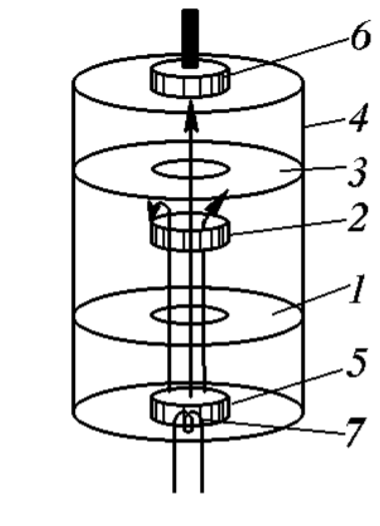
\includegraphics[width=0.18\textwidth]{2.png}}}
    \subfloat{{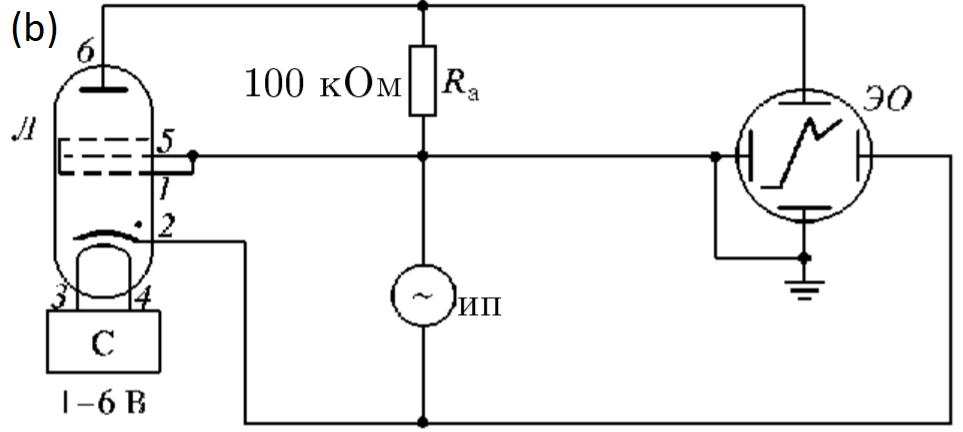
\includegraphics[width=0.5\textwidth]{3.png}}}
  \centering
  \caption{(a) Схема тиратрона (слева) и его конструкция (справа): 1,2,3 -- сетки, 4 -- внешний металлический цилиндр, 5 -- катод, 6 -- анод, 7 -- накаливаемая спираль. (b) Схема включения тиратрона.}
\end{figure}
Для изучения эффекта испульзуется тиратрон ТГ3-01/1.3Б, заполненный инертным газом (Рис. 1а). Электроны эмитируются катодом, ускоряются напряжением $V$ и рассеиваются на атомах газа(ксенона). Сетки соединены между собой и имеют один потенциал, примерно равный потенциалу анода. Рассеянные электроны отклоняются и уходят на сетку, а оставшиеся достигают анода, создавая ток $I_\text{a}$. Таким образом, поток электронов на расстоянии $x$ от ускоряющей сетки уменьшается с ростом $x$. ВАХ анода должна быть
\begin{equation}\label{3}
I_\text{a} = I_0 \exp\left( - C w(V) \right),
\end{equation}
где $I_0 = eN_0$ -- ток катода, $I_\text{a} = eN_a$ -- ток анода, $C = Ln_\text{a} \Delta_\text{a}$($L$ --  расстояние между катодом и анодом, $\Delta_\text{a}$ -- площадь поперечного сечения атома, $n_\text{a}$ -- концентрация газа в лампе), $w(V)$ -- вероятность рассеяния на атоме.
Формулу \eqref{3} можно переписать в виде
\[\tag{5a}\label{5a}
w(V) = -\dfrac{1}{C}\ln \dfrac{I_\text{a}(V)}{I_0}.
\]
\begin{figure}[H]
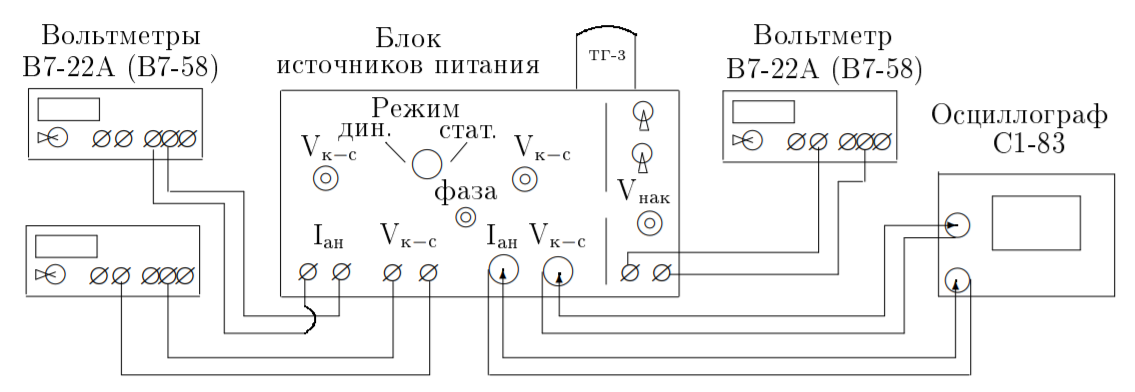
\includegraphics[scale=0.5]{1.png}
\centering
\caption{Схема установки.}
\end{figure}

\section{Ход работы}
\begin{enumerate}
  \item Подключили схему к сети переменного тока $220В$ (частота $50 Гц$).
  \item Вначале напряжение накала установили на уровне $2 - 2,5 В$, осциллограф - в режиме внешней развертки.
  \item Плавно увеличивая подавая от генератона на тиратрон напряжение, наблюдали ВАХ тиратрона.
  \item Поднеся к лампе постоянный магнит, убедились, что магнитное поле обостряет эффект Размауэра.
  \item Провели измерения ВАХ тиратрона на двух значениях напряжения накала.

  \begin{table}[H]
    \centering
    \begin{tabular}{|l|l|l|l|}
      \hline
    Unak, B & Vmax, B & Vmin, B & Vpr, B \\ \hline
    2,6   & 1,6     & 7,2     & 11,4   \\ \hline
    2,3   & 1,5    & 6,0       & 13,6 \\ \hline
    \end{tabular}
    \caption{Измерения, проведенные с помощью ЭО.}
    \end{table}

    \begin{table}[H]
      \begin{tabular}{|l|l|l|l|l|l|l|l|l|l|l|l|l|l|l|}
    \hline
      V, B  & 0,60 & 0,71 & 0,81 & 0,92 & 1,00 & 1,12 & 1,20  & 1,31  & 1,42  & 1,52 & 1,60 & 1,71 & 1,81 & 1,91 \\ \hline
    I, мA & 0,00                         & 0,00                         & 0,00 & 0,02 & 0,05 & 0,13 & 0,21  & 0,34  & 0,45  & 0,52 & 0,53 & 0,52 & 0,51 & 0,46 \\ \hline
    V, B  & 2,01                         & 2,13                         & 2,21 & 2,30 & 2,46 & 2,50 & 2,60  & 2,71  & 2,81  & 2,92 & 3,01 & 3,13 & 3,22 & 3,31 \\ \hline
    I, мA & 0,44                         & 0,40                         & 0,38 & 0,35 & 0,30 & 0,29 & 0,26  & 0,23  & 0,21  & 0,19 & 0,18 & 0,17 & 0,16 & 0,15 \\ \hline
    V, B  & 3,40                         & 3,51                         & 3,63 & 3,71 & 3,82 & 3,92 & 4,01  & 4,11  & 4,20  & 4,32 & 4,41 & 4,62 & 4,86 & 4,95 \\ \hline
    I, мA & 0,15                         & 0,14                         & 0,13 & 0,12 & 0,12 & 0,11 & 0,11  & 0,10  & 0,10  & 0,10 & 0,10 & 0,09 & 0,09 & 0,09 \\ \hline
    V, B  & 5,15                         & 5,25                         & 5,40 & 5,59 & 5,77 & 5,94 & 6,24  & 6,56  & 6,90  & 7,20 & 7,57 & 7,70 & 7,90 & 8,25 \\ \hline
    I, мA & 0,08                         & 0,08                         & 0,08 & 0,08 & 0,08 & 0,08 & 0,07  & 0,07  & 0,07  & 0,07 & 0,07 & 0,07 & 0,07 & 0,07 \\ \hline
    V, B  & 8,57                         & 8,80                         & 9,10 & 9,42 & 9,55 & 9,80 & 10,60 & 11,05 & 11,58 &      &      &      &      &      \\ \hline
    I, мA & 0,07                         & 0,08                         & 0,08 & 0,08 & 0,09 & 0,10 & 0,11  & 0,12  & 0,14  &      &      &      &      &     \\ \hline
      \end{tabular}
      \caption{ВАХ титрана при $U_{нак} = 2,303 В$}
      \end{table}

      % Please add the following required packages to your document preamble:
% \usepackage[table,xcdraw]{xcolor}
% If you use beamer only pass "xcolor=table" option, i.e. \documentclass[xcolor=table]{beamer}
\begin{table}[H]
  \begin{tabular}{|l|l|l|l|l|l|l|l|l|l|l|l|l|l|l|}
    \hline
  V, B  & 0,43 & 0,50 & 0,61 & 0,72 & 0,74 & 0,75 & 0,81 & 0,86 & 0,91 & 0,96  & 1,06  & 1,10  & 1,16 & 1,22 \\ \hline
  I, мA & 0,00                         & 0,00                         & 0,00 & 0,01 & 0,01 & 0,02 & 0,02 & 0,06 & 0,09 & 0,15  & 0,30  & 0,38  & 0,51 & 0,67 \\ \hline
  V, B  & 1,28                         & 1,36                         & 1,42 & 1,48 & 1,50 & 1,54 & 1,58 & 1,64 & 1,80 & 1,85  & 1,96  & 2,00  & 2,10 & 2,22 \\ \hline
  I, мA & 0,82                         & 1,02                         & 1,14 & 1,27 & 1,31 & 1,37 & 1,43 & 1,49 & 1,58 & 1,58  & 1,56  & 1,55  & 1,51 & 1,44 \\ \hline
  V, B  & 2,31                         & 2,45                         & 2,71 & 2,87 & 3,01 & 3,30 & 3,55 & 3,69 & 3,93 & 4,05  & 4,24  & 4,53  & 4,84 & 5,04 \\ \hline
  I, мA & 1,38                         & 1,30                         & 1,13 & 1,05 & 0,95 & 0,81 & 0,72 & 0,68 & 0,63 & 0,60  & 0,57  & 0,53  & 0,49 & 0,47 \\ \hline
  V, B  & 5,33                         & 5,69                         & 5,90 & 6,70 & 7,20 & 7,60 & 8,10 & 8,81 & 9,46 & 10,07 & 10,75 & 11,45 &      &      \\ \hline
  I, мA & 0,44                         & 0,42                         & 0,42 & 0,40 & 0,40 & 0,40 & 0,42 & 0,46 & 0,51 & 0,67  & 0,71  & 0,89  &      &     \\ \hline
  \end{tabular}
  \caption{ВАХ титрана при $U_{нак} = 2,608 В$}
  \end{table}
\end{enumerate}



\section{Обработка результатов}

\begin{enumerate}
  \item Построим ВАХ тиратрона при разных напряжениях накала.
  \begin{figure}[h]
    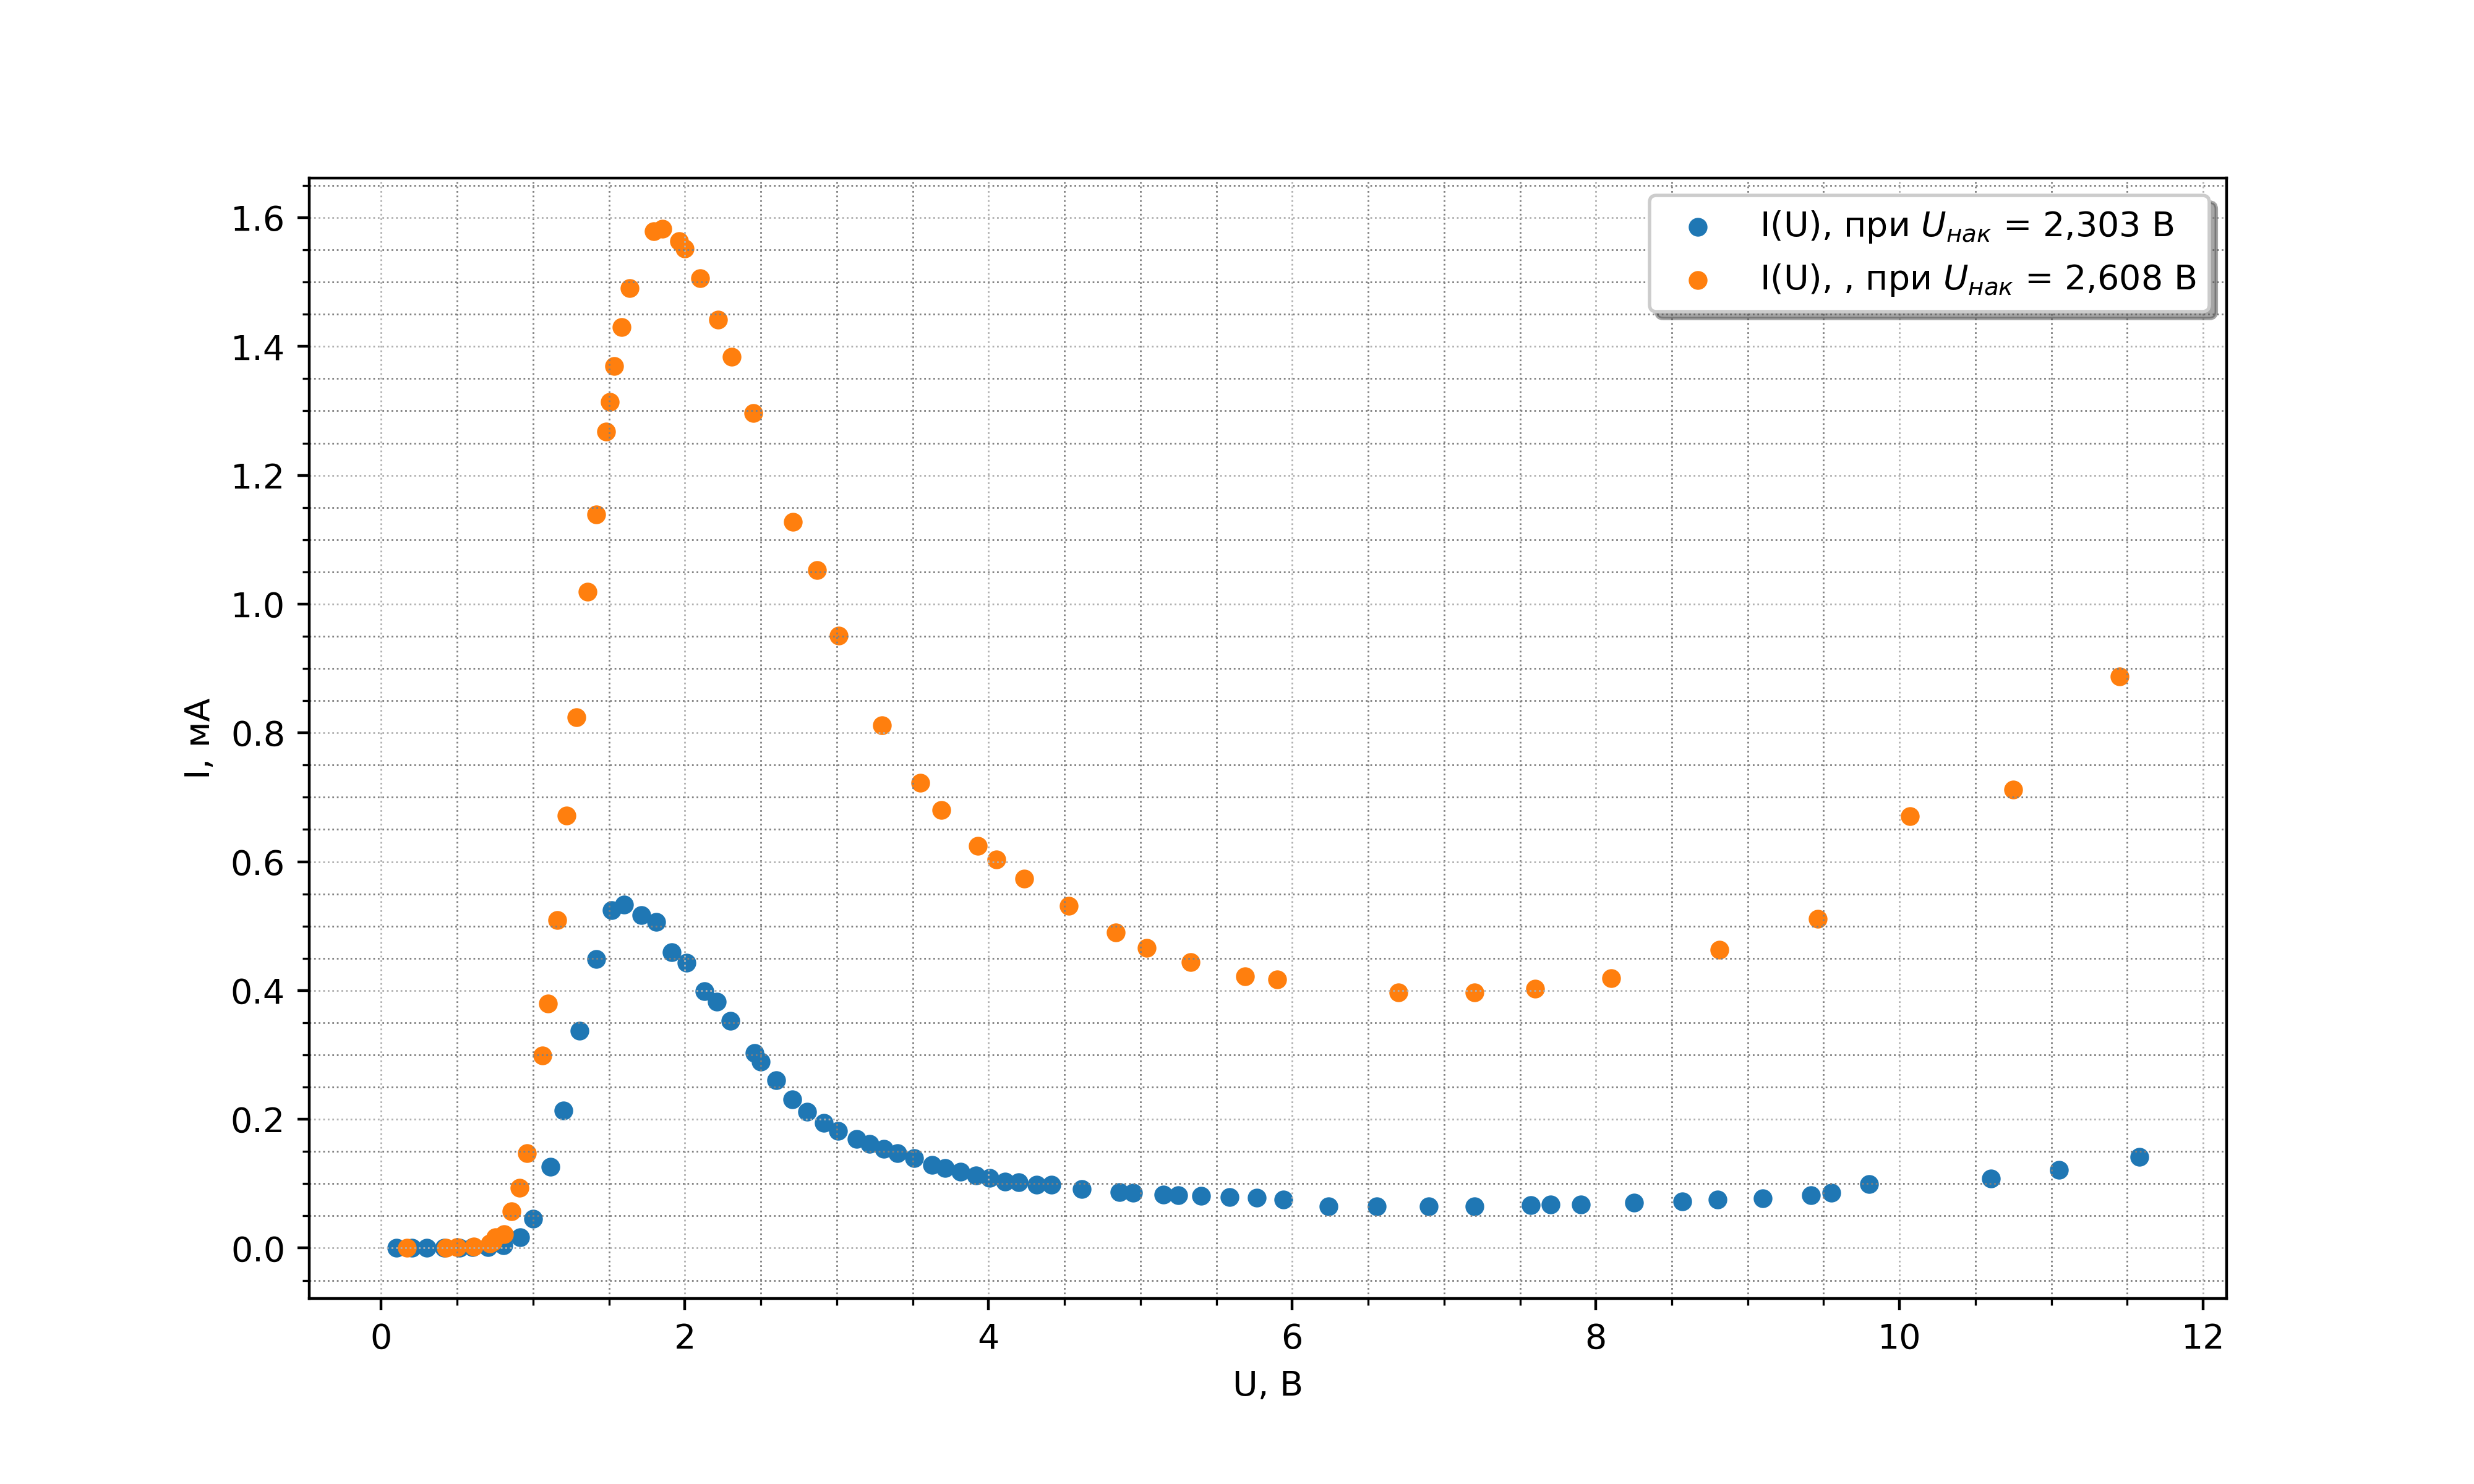
\includegraphics[width=0.8\textwidth]{I(U).png}
    \centering
    \caption{ВАХ титратрона при разных напряжениях накала.}
    \end{figure}
    \item По напряжению пробоя убеждаемся, что тиратрон наполнен ксеноном, чье напряжение ионизации составляет $12,1$ эВ.
    \item Считаем $U_0 = 2,5 эВ$, а $\ell$ найдем из формул \eqref{1}, причем $l_{теор} = 108$пм. \\
    $l_1 = 111,9 \pm 2,4$пм, отличается от теоретического почти на 4$\%$. \\
    $l_2 = 108,5 \pm 2,4$пм, отлично сходится в пределах погрешности. \\

    \item Рассчитаем также по формуле \eqref{2} \\
    $ l = 124,1 \pm 2,7$пм, отличается от теоретического на 15$\%$.
    \item Из формулы \eqref{0} оценим значения напряжений максимумов порядка $n > 2$:
    \[E_2= 16.7~\text{эВ},~E_3 = 40.7~\text{эВ},~E_4 = 74.3~\text{эВ}.\]
    Полученные энергии выше потенциала ионизации, поэтому эти максимумы уже не будут наблюдаться.
    
    \item Наконец, в соответствии с \eqref{5a}, можно получит качественную зависимость вероятности рассеяния от напряжения на титротроне. 
    \begin{figure}[H]
      \subfloat{{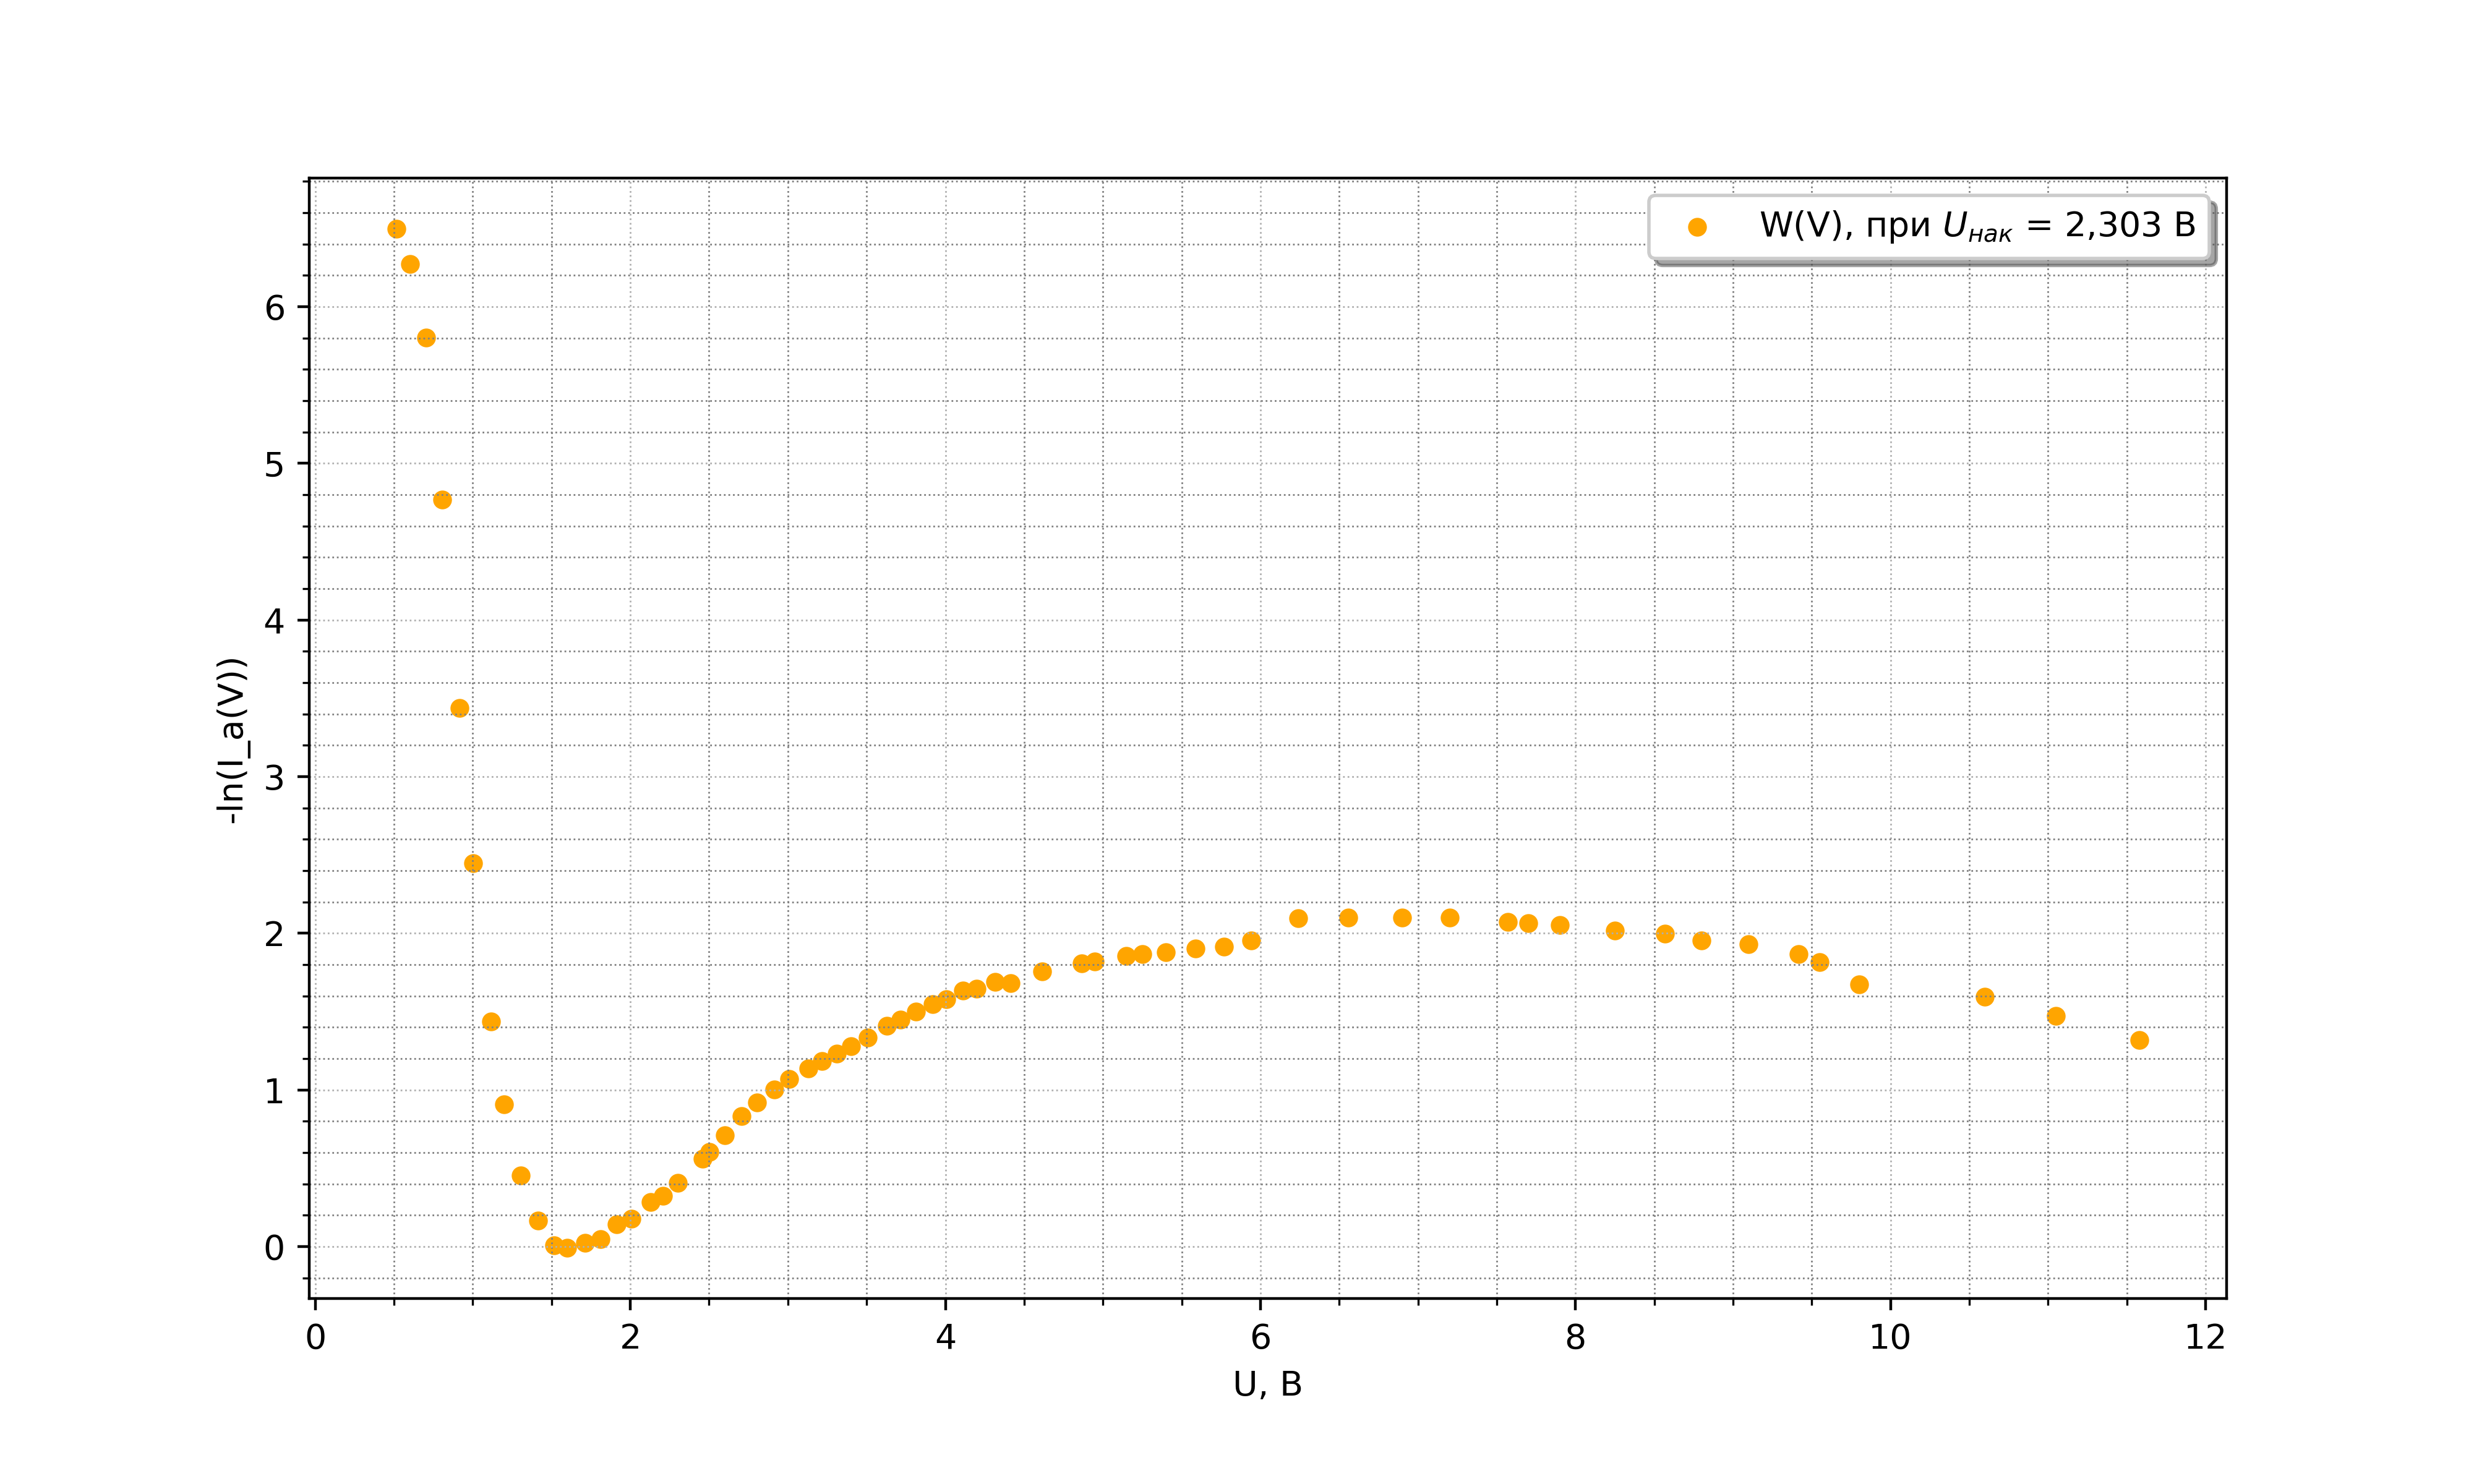
\includegraphics[width=0.49\textwidth]{W1.png}}}
      \subfloat{{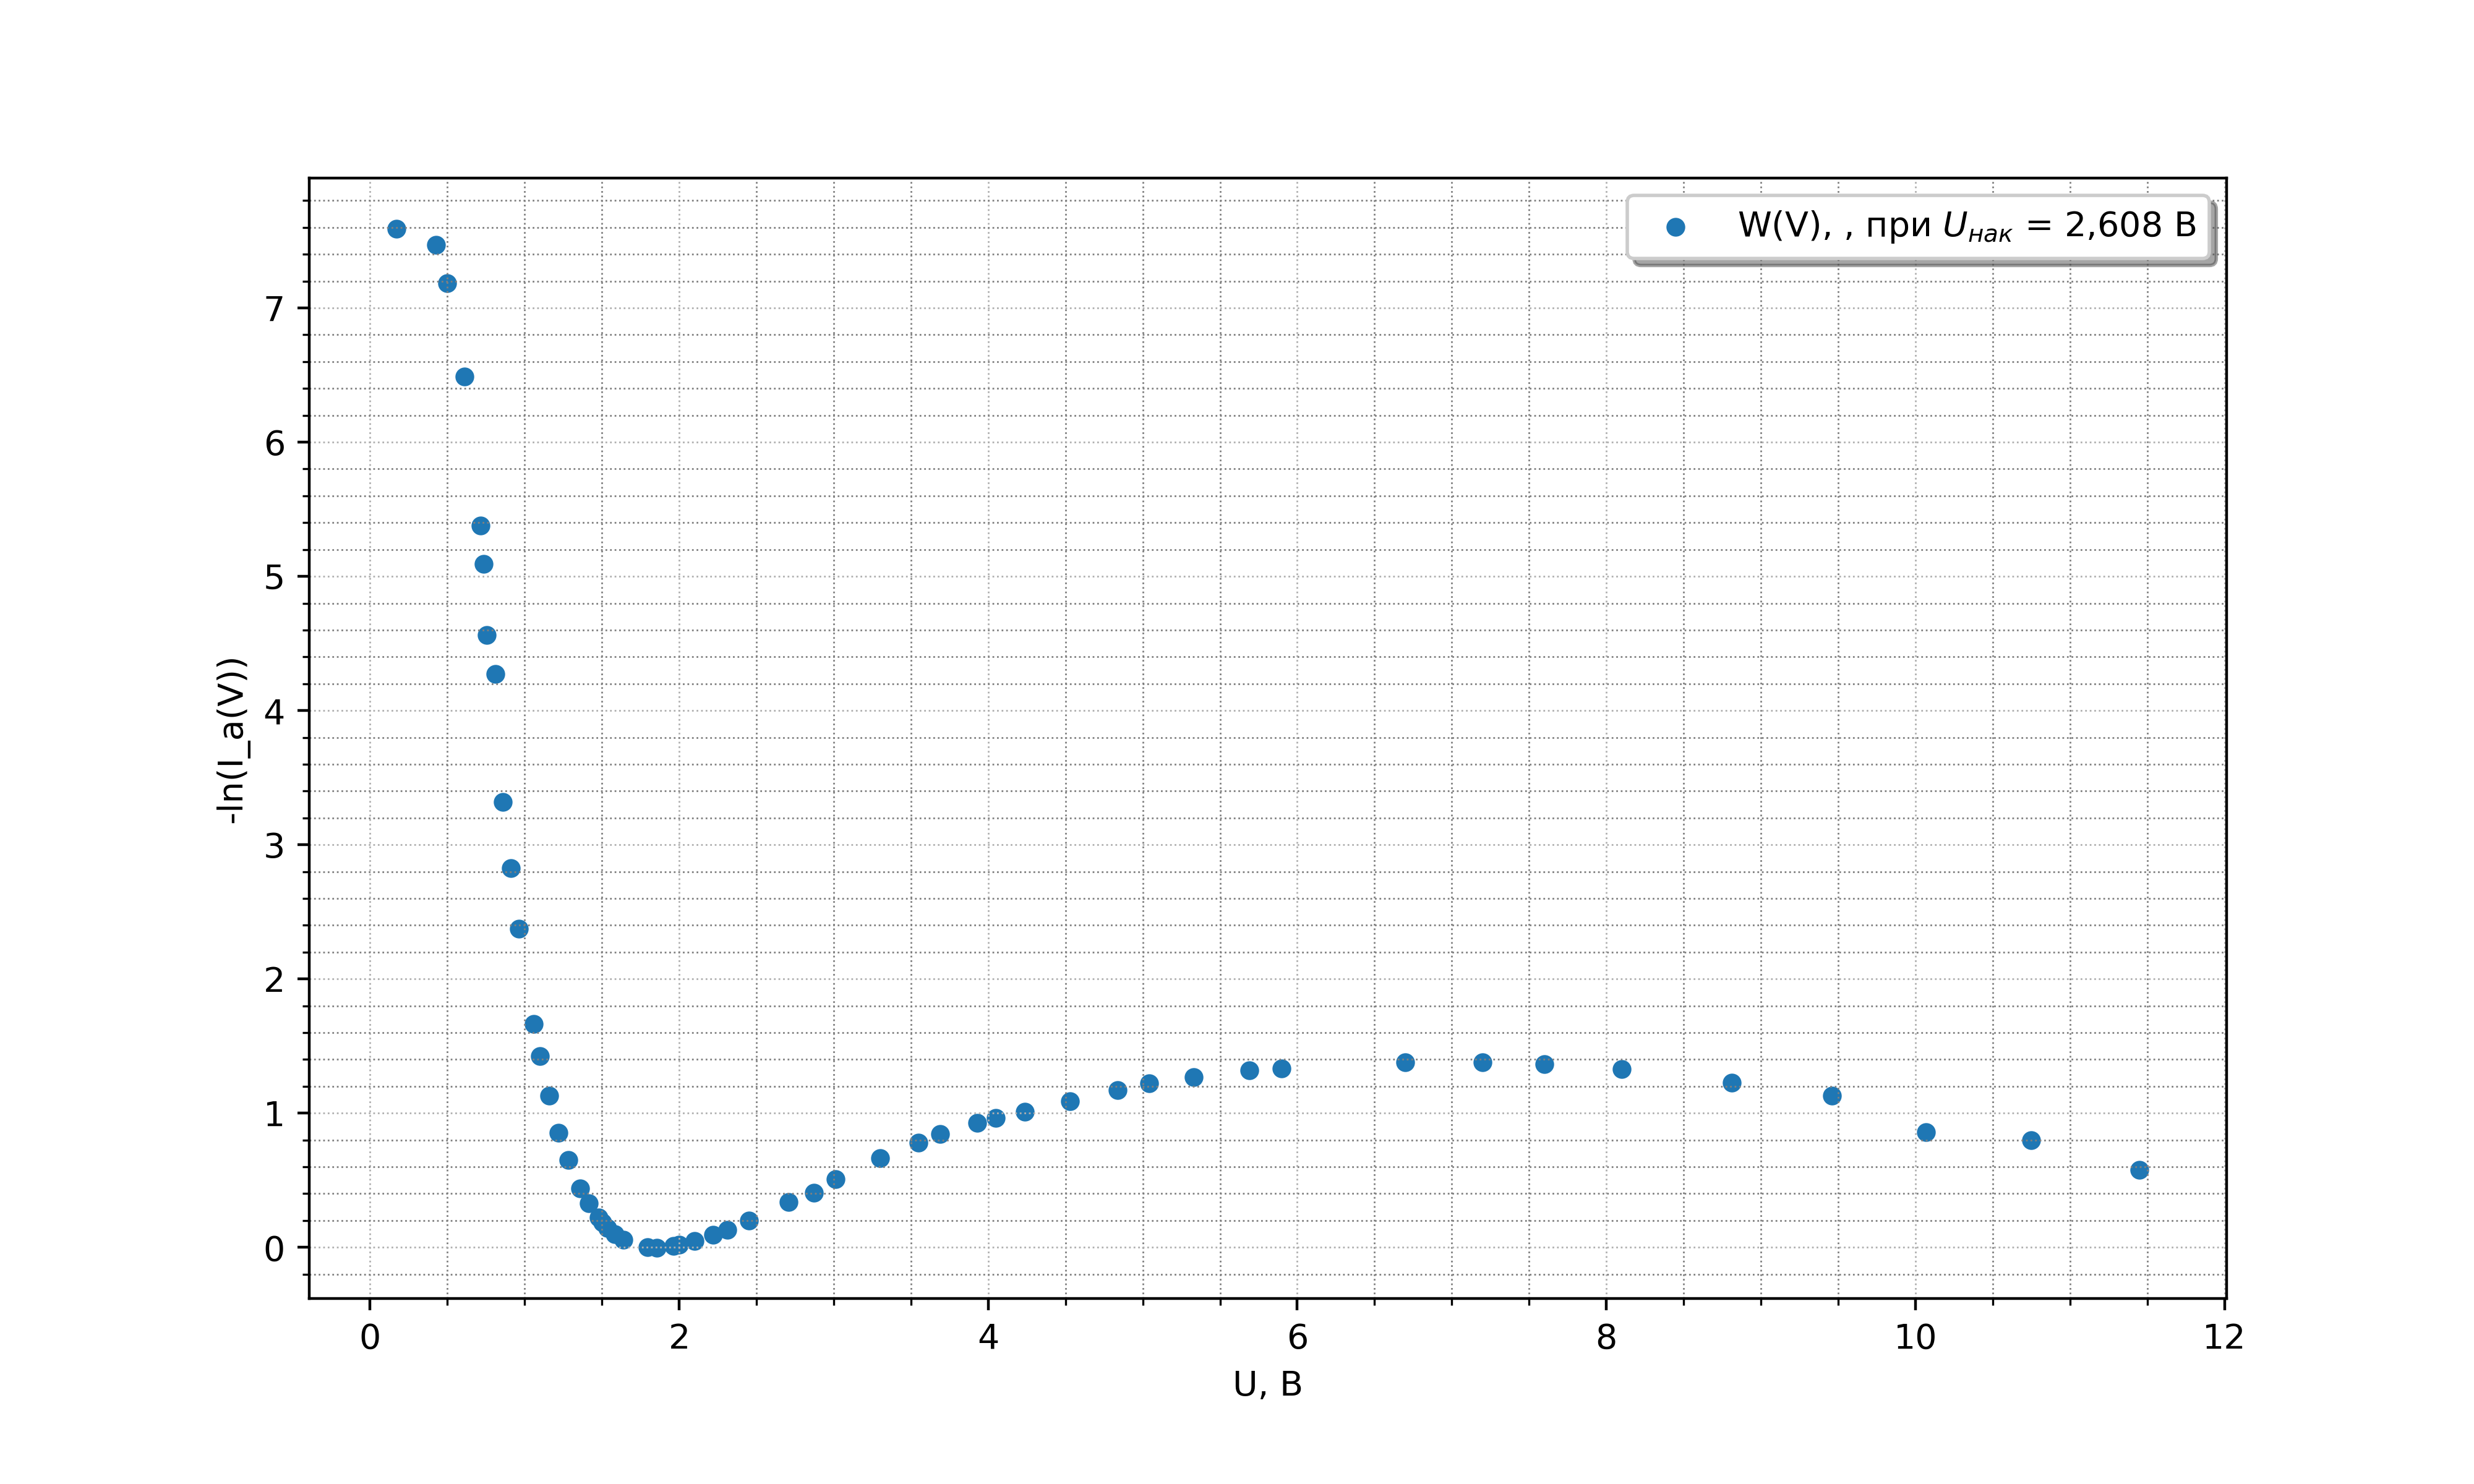
\includegraphics[width=0.49\textwidth]{W2.png}}}
    \centering
    \caption{График качественной зависимости $w(V) = -\frac{1}{C}ln\frac{I_a(V)}{I_0}$}
    \end{figure}
\end{enumerate}



\section{Вывод}
В ходе работы была статическим и динамическим методом исследована ВАХ титратрона, в обоих случаях соответствующая теоретической, получено значение размера внешней оболочки атома инертного газа.

\section{Литература}
Игошин Ф.Ф., Самарский Ю.А., Ципенюк Ю.М. - Лабораторный практикум по общей физике: Учеб. пособие для вузов. Т. 3 Квантовая физика. 
М.: Физматкнига, 2005.

\end{document}